\documentclass[11pt,a4paper]{article}

\usepackage[utf8]{inputenc}
\usepackage[T1]{fontenc}
\usepackage{lmodern}
\usepackage[spanish,es-noshorthands,es-tabla]{babel}
\usepackage[top=2.5cm,bottom=2.5cm,left=2.5cm,right=2.5cm]{geometry}
\usepackage{microtype}
\usepackage{amsmath,amssymb}
\usepackage{graphicx}
\usepackage{booktabs}
\usepackage{array}
\usepackage{float}
\usepackage{xcolor}
\usepackage{caption}
\usepackage{subcaption}
\usepackage{listings}
\usepackage{url}
\usepackage{tikz}
\usetikzlibrary{positioning,arrows.meta,calc,shapes.geometric,fit}
\usepackage[colorlinks=true,linkcolor=navy,urlcolor=navy,citecolor=navy]{hyperref}

\definecolor{navy}{RGB}{11,37,69}
\definecolor{cellblue}{RGB}{19,64,116}
\definecolor{amber}{RGB}{250,176,5}
\definecolor{softgray}{RGB}{245,246,248}
\graphicspath{{../data/processed/}}
\urlstyle{tt}
\newcommand{\ruta}[1]{{\small\path{#1}}}
\emergencystretch=3em
\setlength{\parindent}{0pt}
\setlength{\parskip}{0.7em}
\renewcommand{\arraystretch}{1.15}
\captionsetup{font=small,labelfont=bf,skip=6pt}

\lstdefinestyle{codigo}{
  basicstyle=\ttfamily\footnotesize,
  breaklines=true,
  breakatwhitespace=false,
  columns=fullflexible,
  keepspaces=true,
  frame=single,
  rulecolor=\color{gray!60},
  backgroundcolor=\color{softgray},
  xleftmargin=0.6em,
  xrightmargin=0.6em,
  numbers=left,
  numberstyle=\tiny\color{gray},
  numbersep=6pt,
  commentstyle=\color{gray!80!black}\itshape,
  keywordstyle=\color{navy}\bfseries,
  showstringspaces=false,
  tabsize=4
}
\lstset{style=codigo}
\renewcommand{\lstlistingname}{C\'odigo}

\title{Forecasting de se\~nales IMU con PyTorch\\
       y despliegue MLOps con Triton}
\author{Juan Ulises Calder\'on Huerta}
\date{\today}

\begin{document}
\selectlanguage{spanish}

\begin{titlepage}
\thispagestyle{empty}
\pagestyle{empty}
\begin{tikzpicture}[remember picture,overlay]
  \fill[navy] (current page.south west) rectangle (current page.north east);
  \begin{scope}
    \clip (current page.south west) rectangle (current page.north east);
    \foreach \i in {0,...,9}{
      \foreach \j in {0,...,14}{
        \pgfmathsetmacro{\x}{\i*2.1}
        \pgfmathsetmacro{\y}{\j*2.1}
        \fill[cellblue,opacity=0.55]
          ($(current page.south west)+(\x+0.06,\y+0.06)$) rectangle
          ($(current page.south west)+(\x+2.04,\y+2.04)$);
        \draw[white,opacity=0.10,line width=0.4pt]
          ($(current page.south west)+(\x+0.7,\y+0.06)$) --
          ($(current page.south west)+(\x+0.7,\y+2.04)$);
        \draw[white,opacity=0.10,line width=0.4pt]
          ($(current page.south west)+(\x+1.4,\y+0.06)$) --
          ($(current page.south west)+(\x+1.4,\y+2.04)$);
      }
    }
  \end{scope}
  \fill[navy,opacity=0.92]
    ($(current page.north west)+(0,-4.6cm)$) rectangle (current page.north east);
  \fill[amber]
    ($(current page.north west)+(0,-4.6cm)$) rectangle
    ($(current page.north east)+(0,-4.75cm)$);
  \node[anchor=north west,text=white,align=left,text width=12cm,font=\sffamily]
    at ($(current page.north west)+(2.2cm,-1.7cm)$)
    {{\large\bfseries\textls*[150]{UNIVERSIDAD DE GUANAJUATO}}\\[3pt]
     {\normalsize Deep Learning}};
  \node[anchor=west,text=white,align=left,text width=15.5cm,font=\sffamily]
    at ($(current page.west)+(2.2cm,3.3cm)$)
    {{\fontsize{31}{36}\selectfont\bfseries Pr\'actica 2:\\
      Forecasting de IMU}\\[14pt]
     {\Large Predicci\'on temporal con RNN y LSTM\\
      y despliegue con Triton}};
  \fill[amber] ($(current page.west)+(2.2cm,0.2cm)$) rectangle ++(3.2cm,0.12cm);
  \node[anchor=north west,text=white!85!navy,align=left,text width=13.5cm,font=\sffamily\small]
    at ($(current page.west)+(2.2cm,-0.2cm)$)
    {Forecasting de seis se\~nales inerciales del dataset EuRoC MAV,
     integraci\'on cinem\'atica de trayectoria y observabilidad MLOps.};
  \fill[white]
    (current page.south west) rectangle ($(current page.south east)+(0,6.6cm)$);
  \fill[amber]
    ($(current page.south west)+(0,6.6cm)$) rectangle
    ($(current page.south east)+(0,6.72cm)$);
  \node[anchor=north west,text=navy,align=left,text width=11cm,font=\sffamily]
    at ($(current page.south west)+(2.2cm,5.7cm)$)
    {{\small\color{gray}\textsc{Autor}}\\[2pt]
     {\Large\bfseries Juan Ulises Calder\'on Huerta}\\[10pt]
     {\small\color{gray}\textsc{Instituci\'on}}\\[2pt]
     {\large Universidad de Guanajuato}};
  \node[anchor=south east,text=navy,align=right,font=\sffamily]
    at ($(current page.south east)+(-2.2cm,1.6cm)$)
    {{\small\color{gray}\textsc{Fecha}}\\[2pt] {\large \today}};
  \node[anchor=south west,text=navy,font=\sffamily\small,align=left]
    at ($(current page.south west)+(2.2cm,1.6cm)$)
    {Reporte t\'ecnico de la Pr\'actica 2\\de Deep Learning};
\end{tikzpicture}
\end{titlepage}
\setcounter{page}{1}
\pagestyle{plain}

\tableofcontents
\clearpage
\listoffigures
\clearpage

\section{Resumen}

Este reporte presenta un sistema de aprendizaje profundo para forecasting
un paso adelante de se\~nales inerciales. A partir de una ventana hist\'orica de
50 muestras, modelos recurrentes RNN y LSTM predicen la siguiente muestra de
seis variables del sensor IMU: tres velocidades angulares del giroscopio y
tres aceleraciones del aceler\'ometro. Los datos provienen del dataset EuRoC
MAV, que tambi\'en proporciona la trayectoria de referencia del veh\'iculo.

El flujo implementado cubre el ciclo completo de machine learning: carga y
normalizaci\'on de datos, ventanas temporales, entrenamiento en PyTorch,
evaluaci\'on, exportaci\'on a ONNX y servicio con Triton Inference Server.
Adem\'as, se realiza una integraci\'on cinem\'atica tipo \emph{strapdown} para
visualizar la deriva acumulada al usar IMU real y predicha. La infraestructura
de despliegue usa Docker Compose, Prometheus y Grafana.

\section{Introducci\'on y objetivos}

La estimaci\'on de movimiento con una unidad de medici\'on inercial permite
obtener informaci\'on de navegaci\'on con alta frecuencia, pero la integraci\'on
de aceleraciones y velocidades angulares acumula error con el tiempo. En este
proyecto se estudia una alternativa complementaria: aprender la din\'amica
local de las se\~nales IMU para predecir la muestra siguiente y observar c\'omo
la predicci\'on afecta la reconstrucci\'on de trayectoria.

Los objetivos son:
\begin{itemize}
  \item Construir un pipeline reproducible de forecasting temporal en PyTorch.
  \item Comparar arquitecturas RNN y LSTM para predecir las seis se\~nales IMU.
  \item Separar cronol\'ogicamente los datos en entrenamiento, validaci\'on y prueba.
  \item Exportar los modelos entrenados a ONNX para inferencia en Triton.
  \item Integrar aceleraci\'on y velocidad angular para visualizar una trayectoria
        2D y su deriva respecto al Ground Truth.
  \item Incorporar observabilidad mediante m\'etricas de Triton, Prometheus y Grafana.
\end{itemize}

\section{Datos y preparaci\'on}

\subsection{Dataset EuRoC MAV}

Se utilizan secuencias del dataset EuRoC MAV, organizadas en carpetas como
\ruta{V1\_01\_easy}, \ruta{V1\_02\_medium} y \ruta{V1\_03\_difficult}. Cada
archivo IMU contiene un timestamp en nanosegundos y las columnas:
\[
\omega_x,\omega_y,\omega_z,a_x,a_y,a_z.
\]
Las velocidades angulares est\'an expresadas en radianes por segundo y las
aceleraciones en metros por segundo al cuadrado. El Ground Truth paralelo
\ruta{state\_groundtruth\_estimate0/data.csv} contiene posici\'on, orientaci\'on
como cuaterni\'on y velocidad en el marco global.

\subsection{Pipeline de ventanas}

El m\'odulo \ruta{src/data\_pipeline.py} divide una secuencia cronol\'ogicamente
con proporciones 70\% para entrenamiento, 15\% para validaci\'on y 15\% para
prueba. El escalador se calcula exclusivamente con el subconjunto de
entrenamiento, evitando filtrar informaci\'on del futuro:
\[
\tilde{x}_{j}=\frac{x_j-\mu_j}{\sigma_j}.
\]
Posteriormente se crean ventanas deslizantes de longitud $L=50$:
\[
X_t=[\tilde{x}_{t-50},\ldots,\tilde{x}_{t-1}],\qquad
y_t=\tilde{x}_t.
\]
Por tanto, la entrada tiene forma $[B,50,6]$ y la salida forma $[B,6]$.
Los par\'ametros $\mu$ y $\sigma$ se persisten en
\ruta{data/processed/scaler.json}.

\begin{table}[H]
\centering
\begin{tabular}{l l}
\toprule
\textbf{Elemento} & \textbf{Configuraci\'on} \\
\midrule
Se\~nales de entrada & 3 gyro + 3 aceler\'ometro \\
Frecuencia aproximada & 200 Hz \\
Ventana hist\'orica & 50 muestras \\
Horizonte & 1 muestra ($t+1$) \\
Split temporal & 70\% / 15\% / 15\% \\
Normalizaci\'on & Z-score calculado en entrenamiento \\
\bottomrule
\end{tabular}
\caption{Configuraci\'on del problema de forecasting.}
\label{tab:datos}
\end{table}

\section{Modelos y entrenamiento}

\subsection{Arquitecturas recurrentes}

La arquitectura RNN usa una capa recurrente tanh de dos capas y una capa
lineal que proyecta el estado oculto final a seis salidas. La LSTM reemplaza
la celda RNN por una memoria con compuertas, manteniendo la misma interfaz
de entrada y salida. En ambos casos se usa \texttt{batch\_first=True}.

\begin{figure}[H]
\centering
\resizebox{\linewidth}{!}{%
\begin{tikzpicture}[
  node distance=0.7cm and 0.9cm,
  blk/.style={draw=navy,rounded corners=3pt,minimum height=1.35cm,
    minimum width=2.5cm,align=center,font=\footnotesize,fill=blue!7,
    line width=0.8pt},
  arr/.style={-{Latex[length=2mm]},thick,navy}]
  \node[blk] (input) {Ventana IMU\\$[B,50,6]$};
  \node[blk,right=of input] (rec) {RNN o LSTM\\2 capas\\$h=64/128$};
  \node[blk,right=of rec] (last) {Estado final\\$[B,h]$};
  \node[blk,right=of last] (fc) {Capa lineal\\$h\rightarrow6$};
  \node[blk,right=of fc] (output) {Predicci\'on\\$[B,6]$};
  \foreach \a/\b in {input/rec,rec/last,last/fc,fc/output}
    {\draw[arr] (\a) -- (\b);}
\end{tikzpicture}}
\caption{Flujo com\'un de las arquitecturas RNN y LSTM.}
\label{fig:arquitectura}
\end{figure}

Los checkpoints presentes muestran que el modelo LSTM fue entrenado con
\texttt{hidden\_dim=128} y dos capas, mientras que el RNN usa
\texttt{hidden\_dim=64} y dos capas. El script de carga detecta estas
dimensiones desde el checkpoint para evitar incompatibilidades.

\subsection{Entrenamiento y exportaci\'on}

El entrenamiento se implementa en \ruta{src/train.py}. Se utiliza MSE como
funci\'on de p\'erdida y Adam como optimizador. El mejor estado se selecciona
por p\'erdida de validaci\'on y se guarda como
\ruta{checkpoints/best\_lstm.pth} o \ruta{checkpoints/best\_rnn.pth}. Al final,
el modelo se exporta a ONNX con eje de batch din\'amico para Triton:

\begin{lstlisting}[language=Python,caption={Contrato de exportaci\'on a ONNX.}]
input_names = ["input"]
output_names = ["output"]
dynamic_axes = {
    "input": {0: "batch_size"},
    "output": {0: "batch_size"},
}
\end{lstlisting}

\section{Evaluaci\'on de forecasting}

El m\'odulo \ruta{src/evaluate.py} carga el checkpoint, ejecuta inferencia sobre
el segmento de prueba, revierte la normalizaci\'on y calcula MSE y MAE globales
y por se\~nal. Tambi\'en genera una gr\'afica con las seis se\~nales, comparando
el valor real con la predicci\'on del modelo.

\begin{figure}[H]
\centering
\begin{subfigure}[t]{0.48\linewidth}
  \centering
  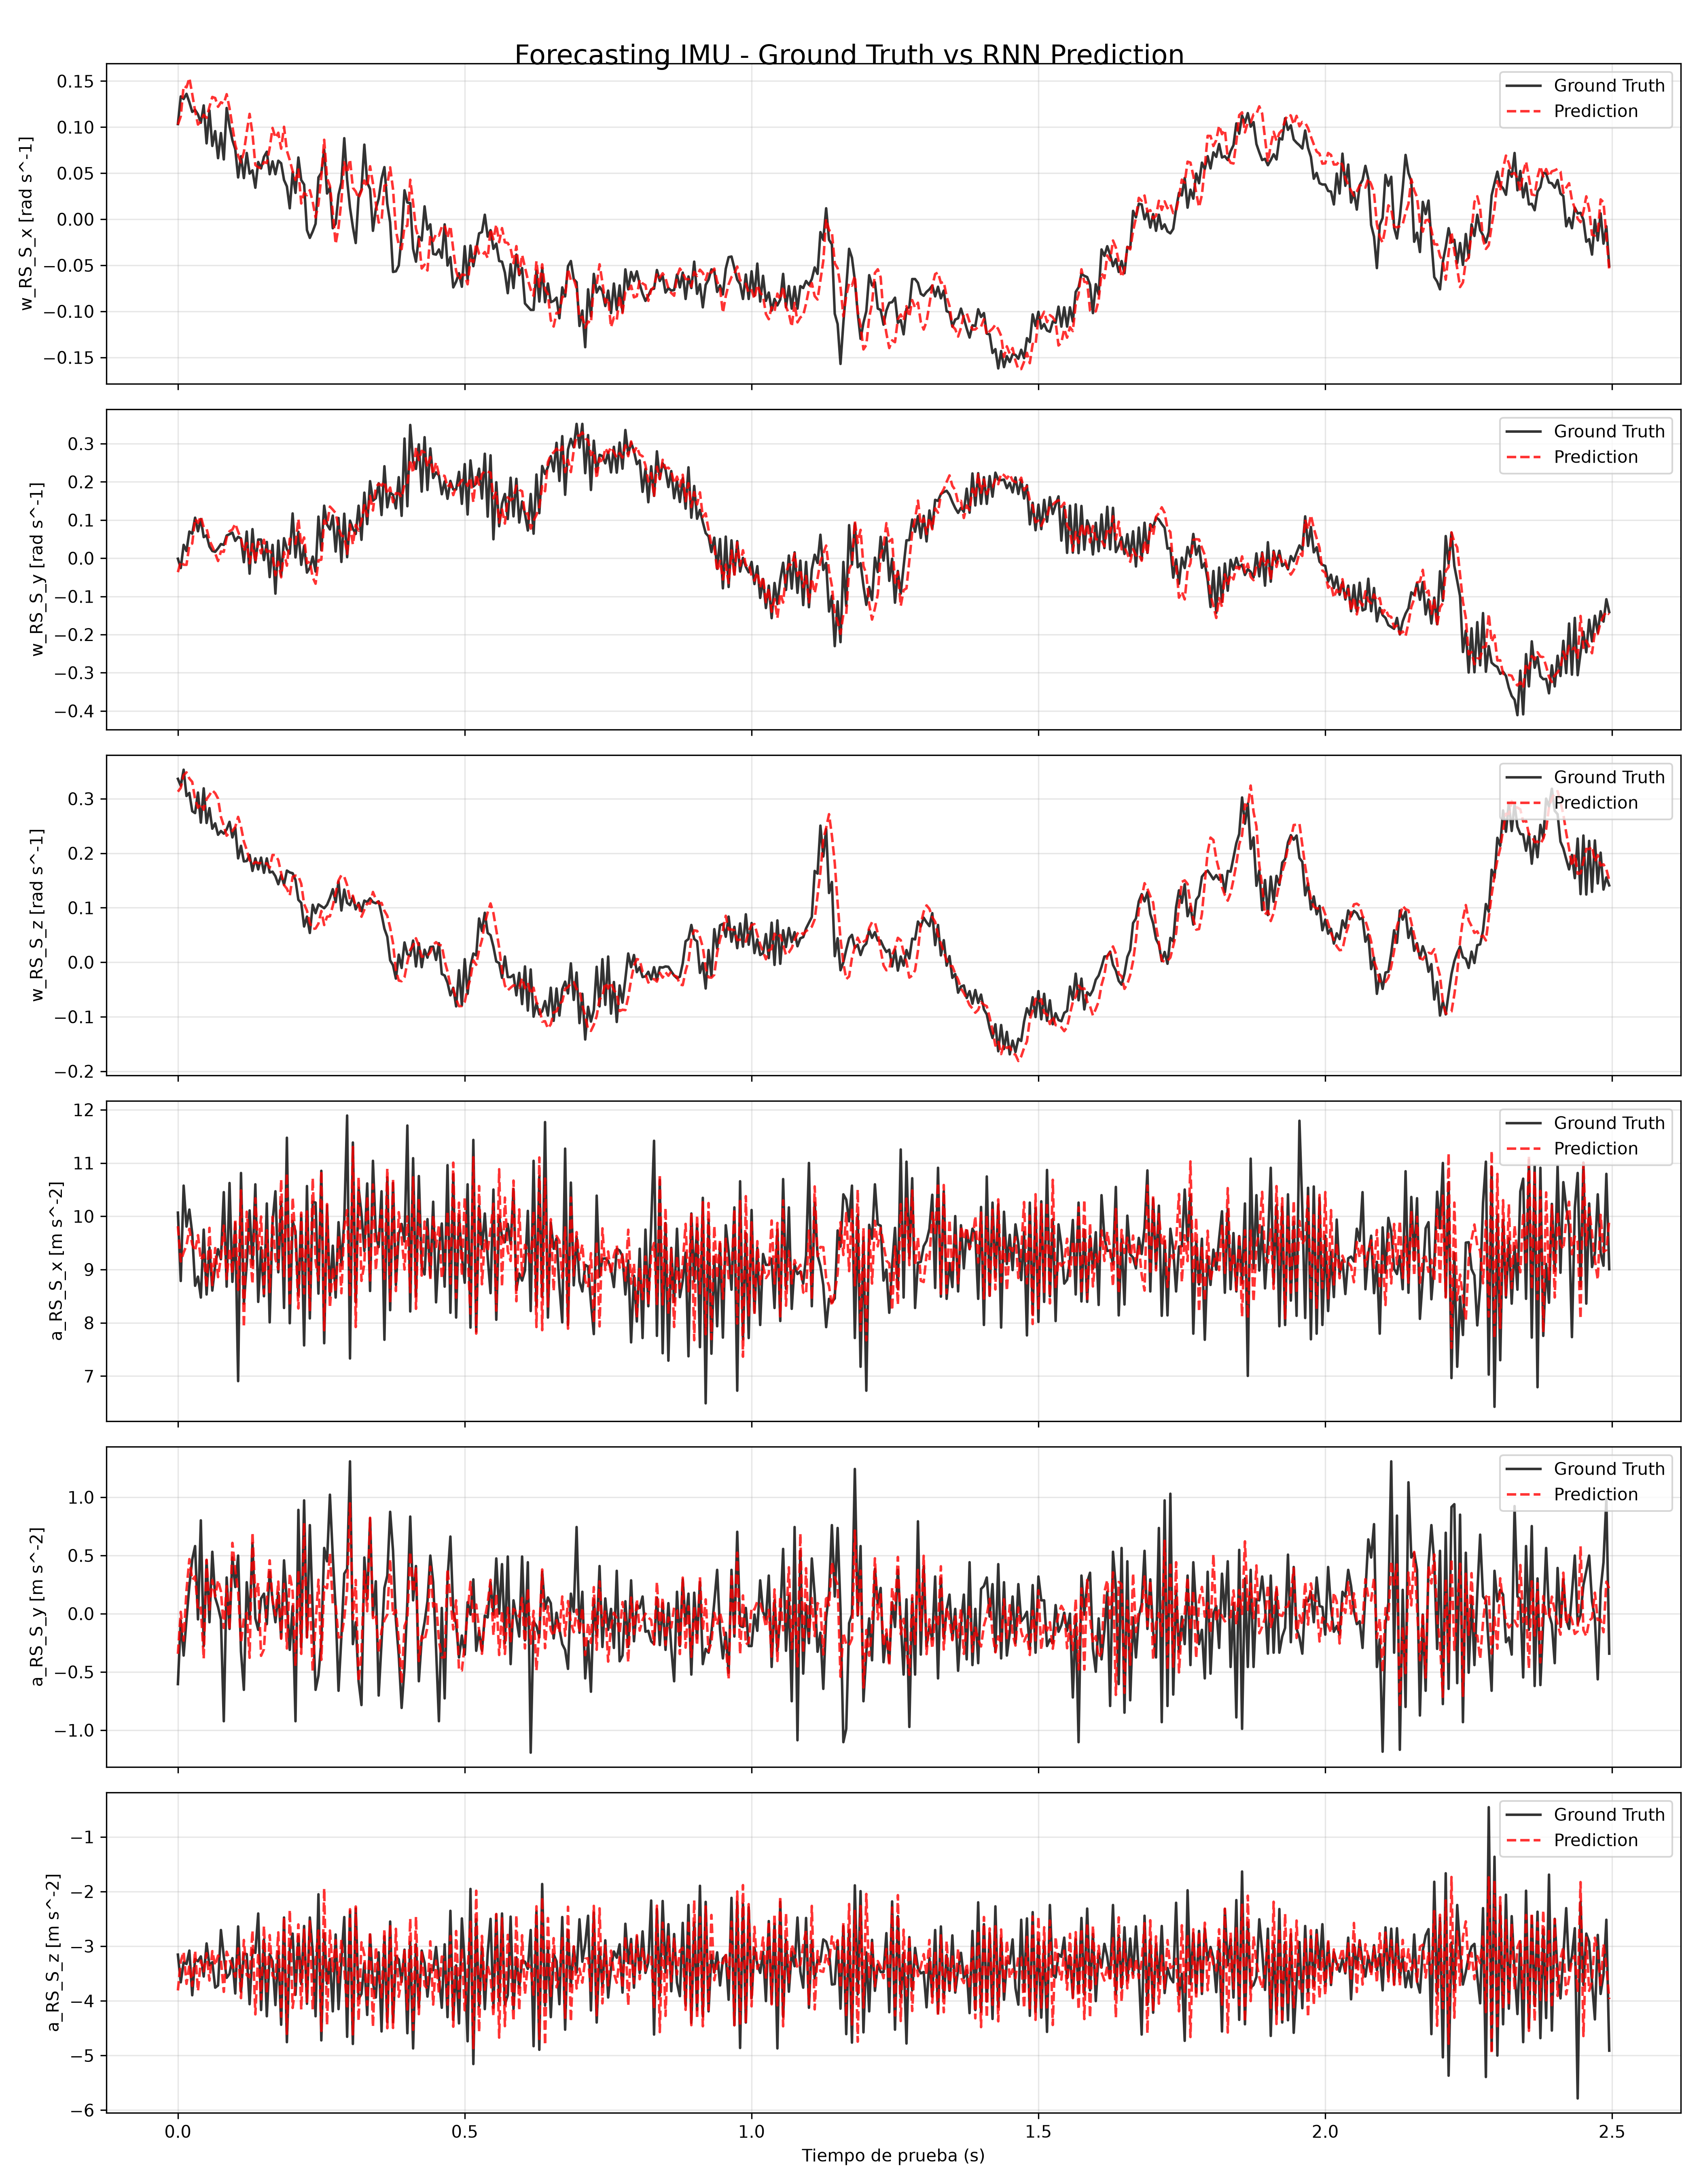
\includegraphics[width=\linewidth,height=0.39\textheight,keepaspectratio]{eval_plot_rnn.png}
  \caption{Predicci\'on del modelo RNN.}
  \label{fig:evalrnn}
\end{subfigure}\hfill
\begin{subfigure}[t]{0.48\linewidth}
  \centering
  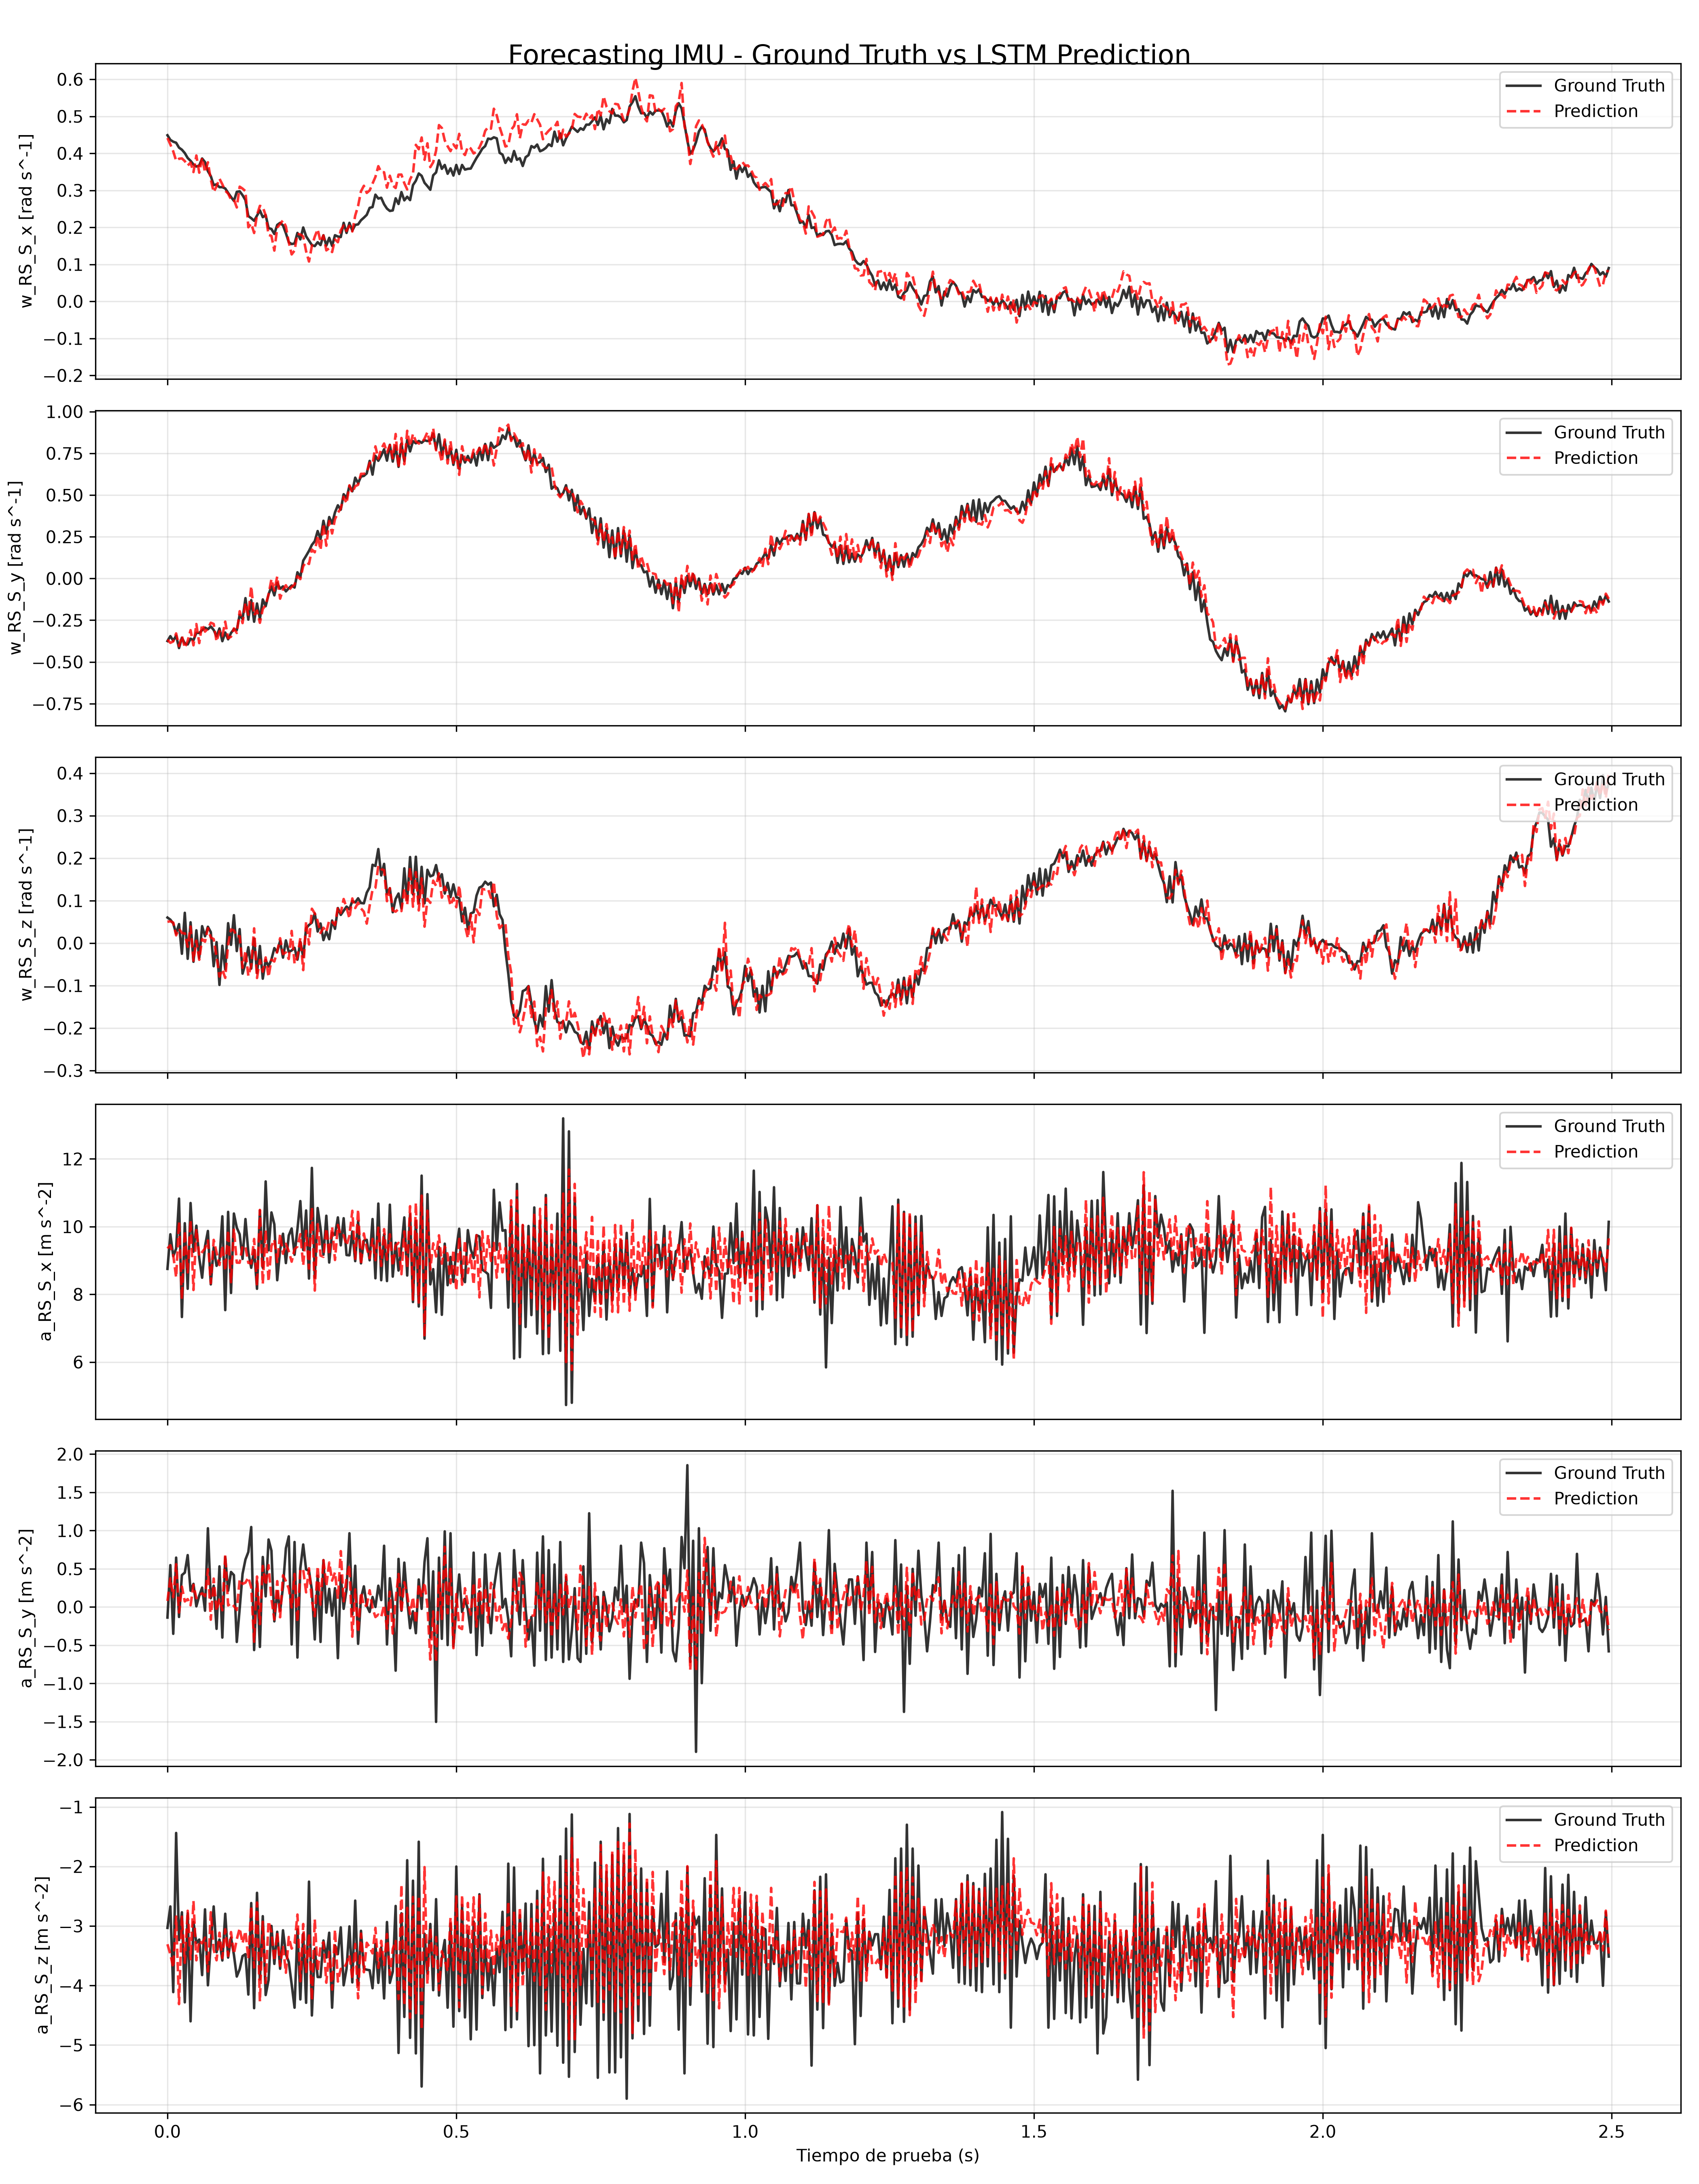
\includegraphics[width=\linewidth,height=0.39\textheight,keepaspectratio]{eval_plot_lstm.png}
  \caption{Predicci\'on del modelo LSTM.}
  \label{fig:evallstm}
\end{subfigure}
\caption{Comparaci\'on de las seis se\~nales IMU en el conjunto de prueba.}
\label{fig:evaluacion}
\end{figure}

Las gr\'aficas muestran que el problema es multivariable: el modelo debe
predecir simult\'aneamente tasas angulares y aceleraciones con escalas f\'isicas
distintas. La normalizaci\'on permite que todas las componentes contribuyan a
la p\'erdida sin que una magnitud domine exclusivamente el entrenamiento.
La evaluaci\'on de un paso no debe confundirse con una garant\'ia de estabilidad
al realizar predicci\'on autoregresiva durante muchos pasos.

\section{Integraci\'on cinem\'atica y trayectoria}

\subsection{Integraci\'on Strapdown}

El script \ruta{src/trajectory\_integration.py} construye una se\~nal h\'ibrida:
usa IMU real durante entrenamiento y validaci\'on, y predicciones autoregresivas
durante prueba. Cada predicci\'on se obtiene con una ventana que incluye las
muestras anteriores y, en Test, tambi\'en las predicciones ya generadas.

Las condiciones iniciales se extraen de la fila de Ground Truth temporalmente
m\'as cercana al primer timestamp de IMU: posici\'on $\mathbf{p}_0$, velocidad
$\mathbf{v}_0$ y cuaterni\'on $\mathbf{q}_0$. En cada paso se actualiza la
orientaci\'on con la velocidad angular:
\[
\mathbf{R}_k=\mathbf{R}_{k-1}
\operatorname{Exp}\left(\boldsymbol{\omega}_k\Delta t\right),
\qquad
\Delta t=\frac{t_k-t_{k-1}}{10^9}.
\]
La aceleraci\'on se transforma del marco del sensor al global y se compensa
la gravedad:
\[
\mathbf{a}^{g}_k=\mathbf{R}_k\mathbf{a}^{s}_k,\qquad
\mathbf{a}^{\mathrm{lin}}_k=\mathbf{a}^{g}_k-[0,0,9.81].
\]
Finalmente se utiliza una actualizaci\'on Euler semi-impl\'icita:
\[
\mathbf{v}_k=\mathbf{v}_{k-1}+\mathbf{a}^{\mathrm{lin}}_k\Delta t,\qquad
\mathbf{p}_k=\mathbf{p}_{k-1}+\mathbf{v}_k\Delta t.
\]
Esta integraci\'on es deliberadamente b\'asica y no incluye calibraci\'on de
bias, fusi\'on con sensores externos ni correcci\'on de deriva.

\subsection{Trayectorias obtenidas}

\begin{figure}[H]
\centering
\begin{subfigure}[t]{0.48\linewidth}
  \centering
  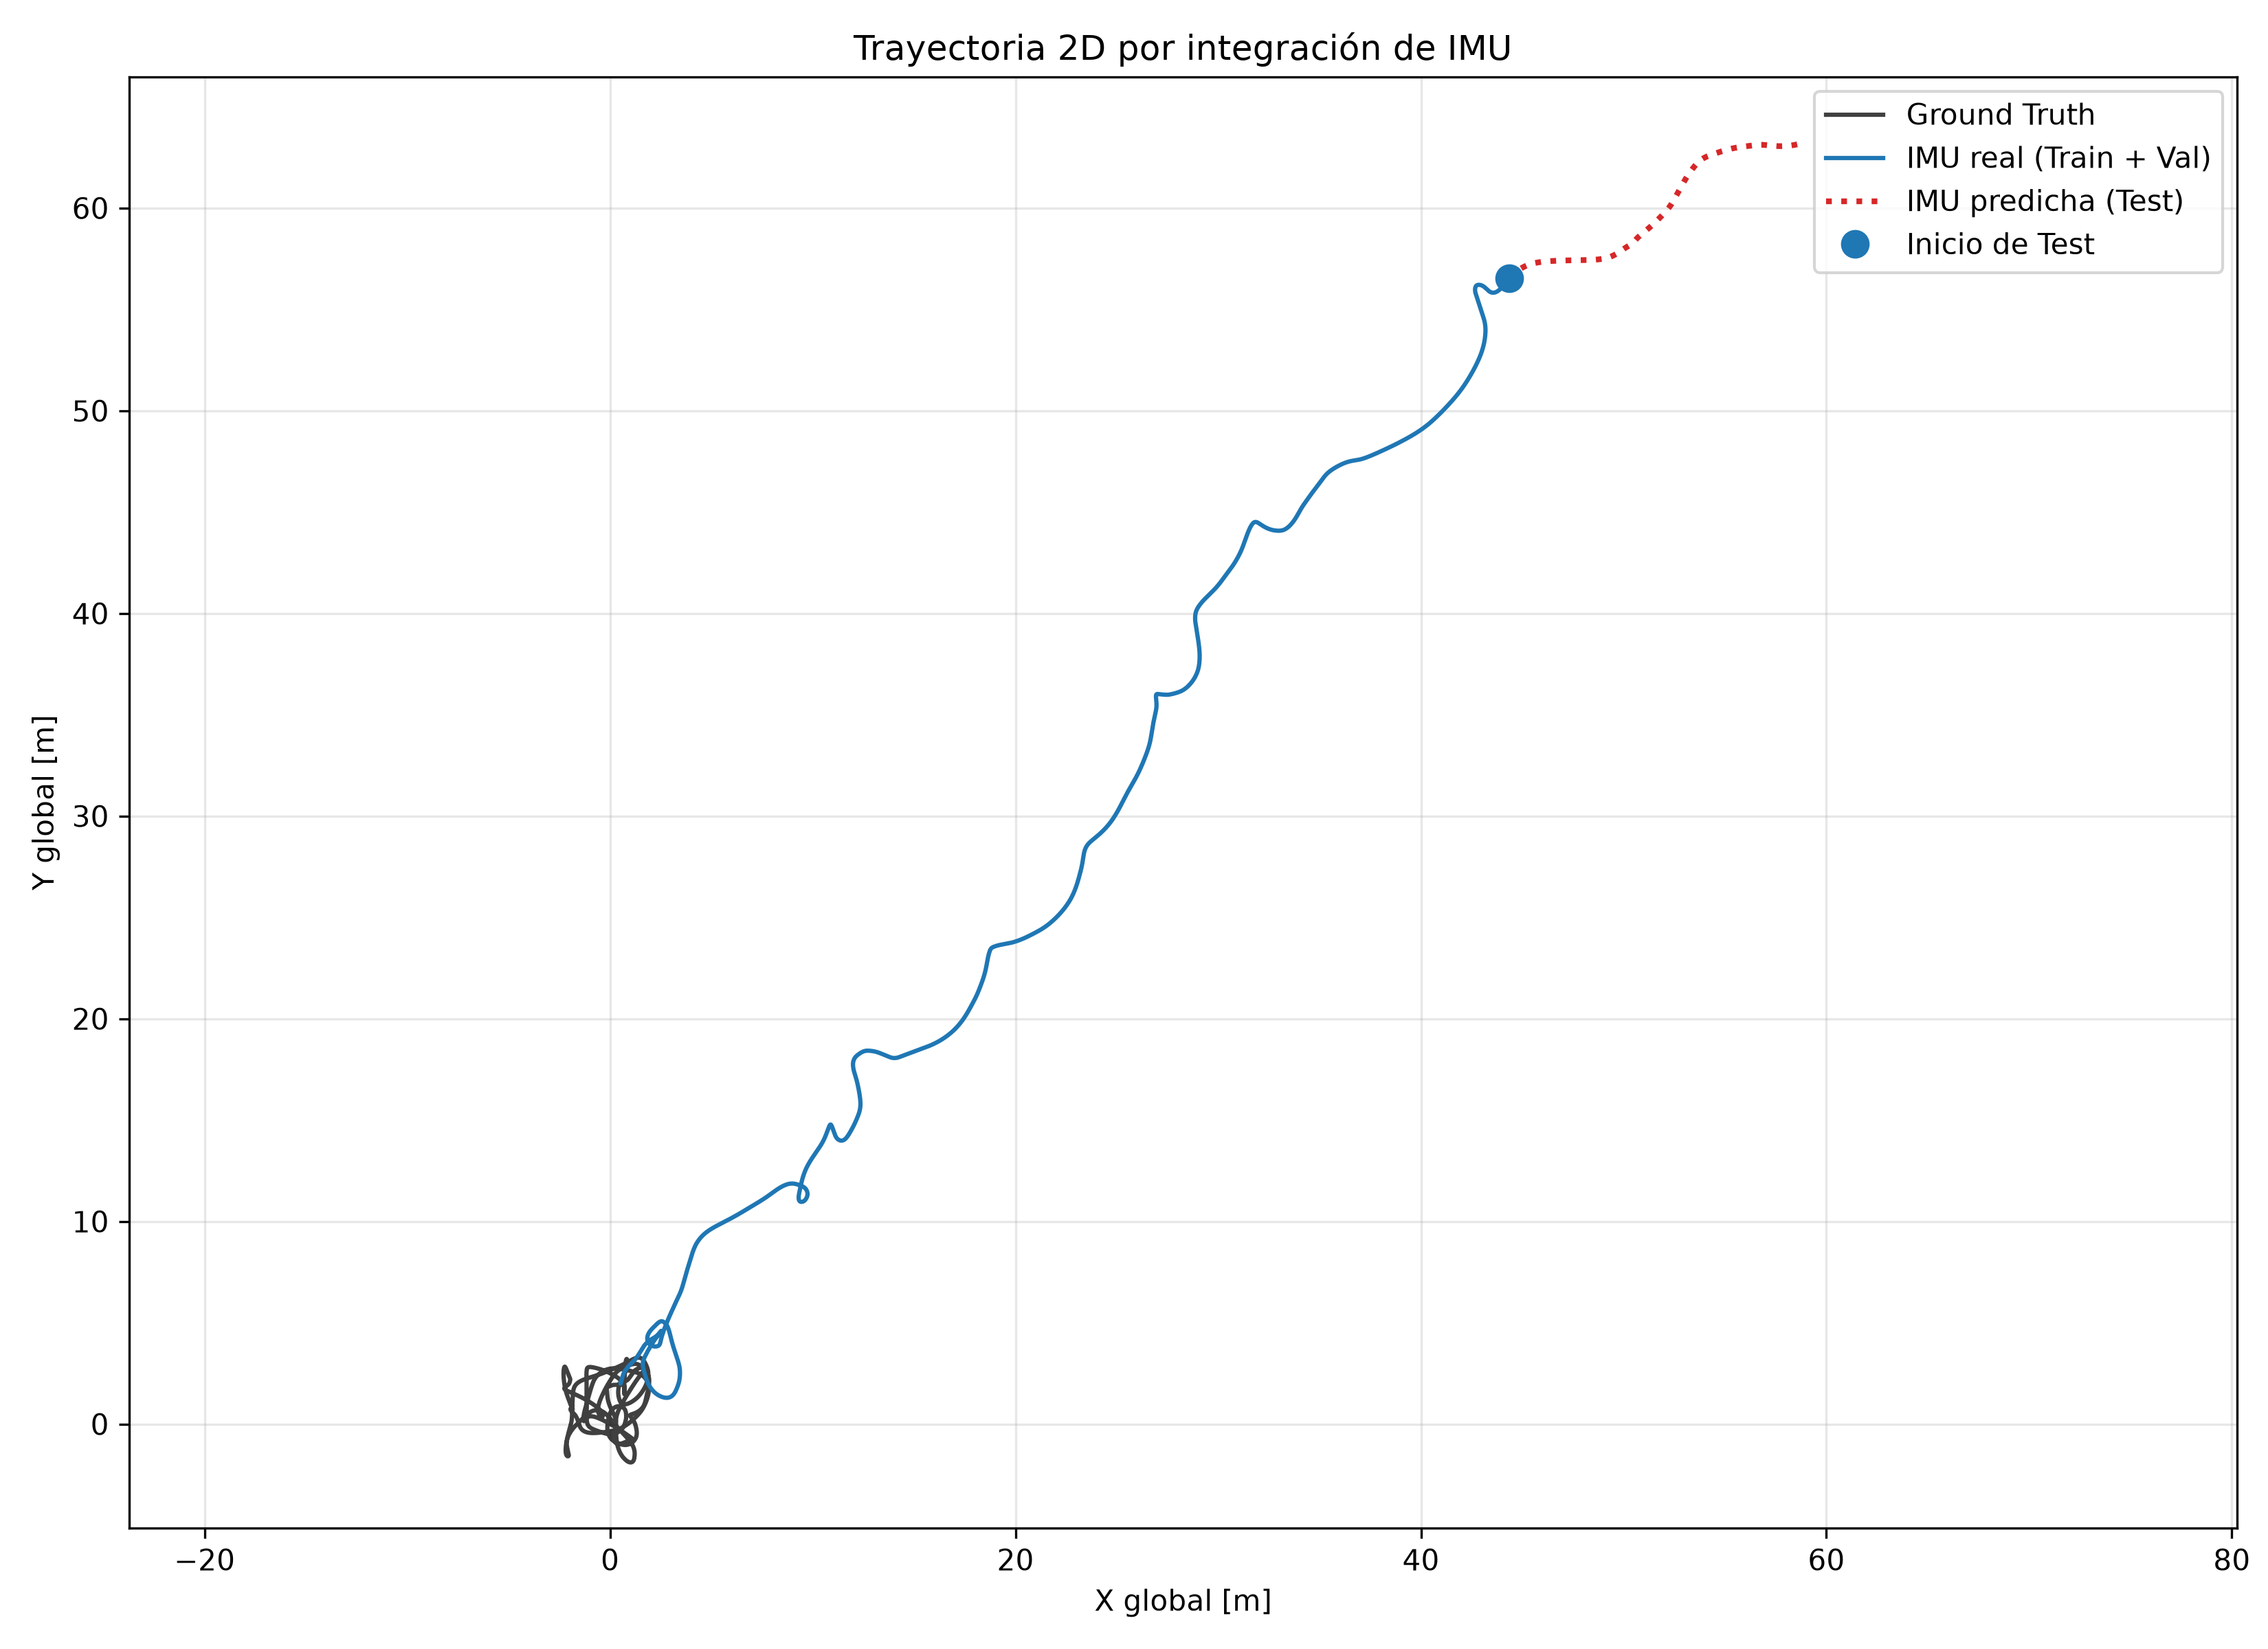
\includegraphics[width=\linewidth,height=0.36\textheight,keepaspectratio]{trajectory_rnn.png}
  \caption{Trayectoria con RNN.}
  \label{fig:trayrnn}
\end{subfigure}\hfill
\begin{subfigure}[t]{0.48\linewidth}
  \centering
  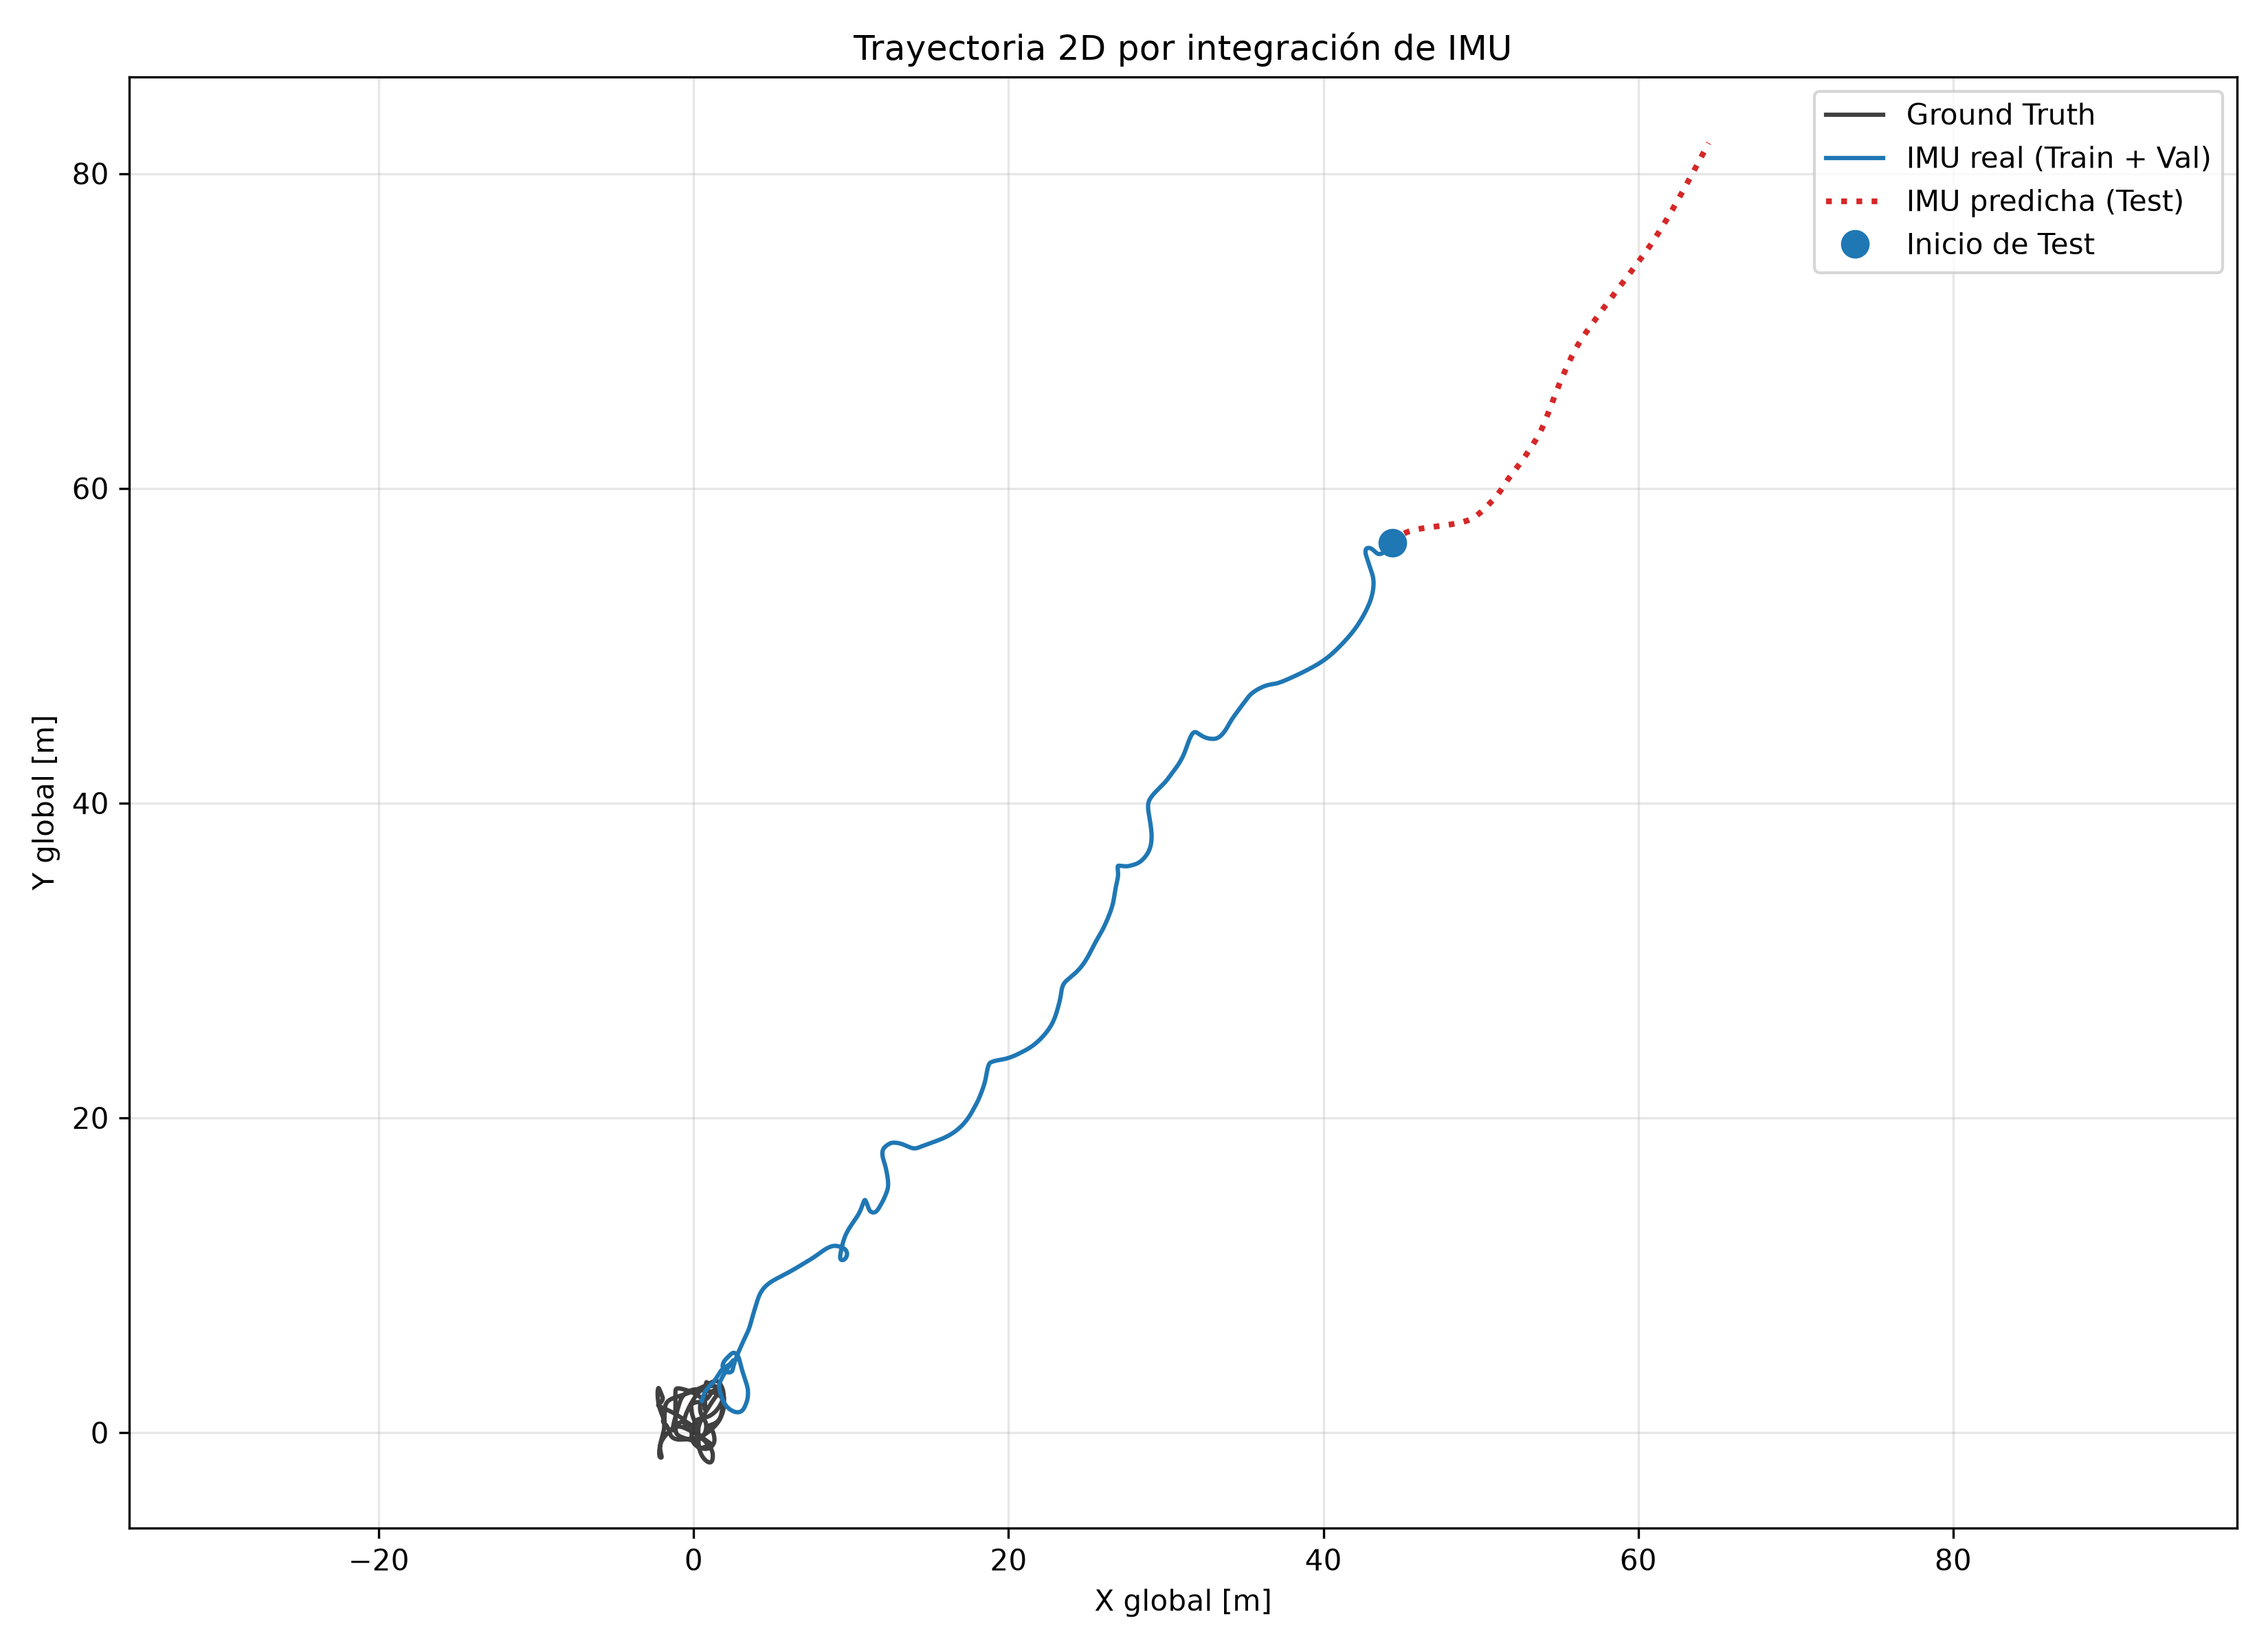
\includegraphics[width=\linewidth,height=0.36\textheight,keepaspectratio]{trajectory_lstm.png}
  \caption{Trayectoria con LSTM.}
  \label{fig:traylstm}
\end{subfigure}
\caption{Vista superior de la trayectoria integrada. Negro: Ground Truth; azul:
IMU real durante Train/Val; rojo punteado: IMU predicha durante Test.}
\label{fig:trayectorias}
\end{figure}

La deriva observada en las curvas estimadas es esperable: un peque\~no error de
aceleraci\'on produce un error creciente en velocidad y un error a\'un mayor en
posici\'on. La visualizaci\'on no pretende reemplazar un sistema de navegaci\'on
inercial calibrado; su prop\'osito es mostrar el efecto acumulativo del error y
la diferencia entre integrar datos reales y datos predichos.

\section{Despliegue MLOps}

\subsection{Repositorio de modelos y Triton}

Los modelos ONNX se organizan con la estructura requerida por Triton:

\begin{lstlisting}[caption={Repositorio de modelos Triton.}]
model_repository/
  lstm_forecaster/
    config.pbtxt
    1/model.onnx
  rnn_forecaster/
    config.pbtxt
    1/model.onnx
\end{lstlisting}

Ambos modelos reciben una entrada \texttt{FP32} de dimensiones $[50,6]$ por
elemento del batch y devuelven seis valores \texttt{FP32}. La configuraci\'on
permite batches de hasta 256 solicitudes y activa \emph{dynamic batching}.
El cliente HTTP en \ruta{src/triton\_client.py} toma un ejemplo normalizado,
construye una entrada $[1,50,6]$ y valida una salida $[1,6]$.

\subsection{Orquestaci\'on y observabilidad}

El archivo \ruta{deploy/docker-compose.yml} levanta tres servicios:
\begin{itemize}
  \item Triton en los puertos HTTP 8000, gRPC 8001 y m\'etricas 8002.
  \item Prometheus en el puerto 9090, haciendo \emph{scrape} de Triton.
  \item Grafana en el puerto 3000 con datasource y dashboard provisionados.
\end{itemize}

\begin{figure}[H]
\centering
\resizebox{\linewidth}{!}{%
\begin{tikzpicture}[
  node distance=0.9cm and 1.0cm,
  blk/.style={draw=navy,rounded corners=3pt,minimum height=1.2cm,
    minimum width=2.7cm,align=center,font=\footnotesize,fill=blue!6,
    line width=0.8pt},
  mon/.style={blk,fill=amber!30},
  arr/.style={-{Latex[length=2mm]},thick,navy},
  darr/.style={-{Latex[length=2mm]},thick,navy,dashed}]
  \node[blk] (client) {Cliente Python\\HTTP};
  \node[blk,right=of client] (triton) {Triton\\RNN / LSTM};
  \node[mon,below=of triton] (prom) {Prometheus\\:9090};
  \node[mon,right=of prom] (graf) {Grafana\\:3000};
  \draw[arr] (client) -- node[above,font=\scriptsize]{inferencia :8000} (triton);
  \draw[darr] (triton) -- node[right,font=\scriptsize]{m\'etricas :8002} (prom);
  \draw[arr] (prom) -- (graf);
\end{tikzpicture}}
\caption{Arquitectura de inferencia y observabilidad del despliegue.}
\label{fig:mlops}
\end{figure}

La imagen de Triton requiere que el host tenga NVIDIA Container Toolkit
configurado cuando se utiliza GPU. La infraestructura est\'a separada del
entorno de entrenamiento para facilitar reproducibilidad y operaci\'on.

\section{Reproducibilidad}

Los pasos principales para reproducir la pr\'actica desde la ra\'iz del
repositorio son:

\begin{lstlisting}[language=bash,caption={Comandos principales del proyecto.}]
conda activate deeplearning
pip install -r requirements.txt
python -m pytest tests/

python src/train.py --model_type lstm \
  --sequence data/raw/V1_01_easy/imu0/data.csv \
  --hidden_dim 128 --num_layers 2

python src/evaluate.py --model_type lstm \
  --sequence data/raw/V1_01_easy/imu0/data.csv

python src/trajectory_integration.py --model_type lstm \
  --sequence data/raw/V1_01_easy/imu0/data.csv

docker compose -f deploy/docker-compose.yml up -d
python src/triton_client.py --model lstm_forecaster
\end{lstlisting}

\section{Limitaciones y trabajo futuro}

\begin{itemize}
  \item La integraci\'on b\'asica no estima bias del aceler\'ometro ni del
        giroscopio; por ello la deriva puede crecer r\'apidamente.
  \item La orientaci\'on se inicializa con Ground Truth, una condici\'on que
        no estar\'ia disponible en un despliegue completamente aut\'onomo.
  \item La evaluaci\'on se realiza sobre una secuencia y un split temporal;
        conviene reportar varias secuencias, semillas y m\'etricas agregadas.
  \item El forecasting autoregresivo puede acumular errores aunque la m\'etrica
        de un paso sea razonable; se requiere evaluar horizontes m\'ultiples.
  \item La integraci\'on podr\'ia mejorarse con preintegraci\'on IMU, filtros
        de Kalman, optimizaci\'on de trayectoria o fusi\'on visual-inercial.
  \item El despliegue MLOps es una demostraci\'on local y no incluye pruebas de
        carga, alta disponibilidad ni autenticaci\'on.
\end{itemize}

\section{Conclusiones}

Se construy\'o un flujo completo para predecir se\~nales IMU con redes
recurrentes y llevar los modelos hasta inferencia servida. El proyecto conecta
el procesamiento temporal de EuRoC MAV con checkpoints PyTorch, exportaci\'on
ONNX, Triton, Prometheus y Grafana. La reconstrucci\'on de trayectoria permite
observar de forma concreta que los errores peque\~nos de las se\~nales inerciales
se acumulan al integrar.

Como resultado de la Pr\'actica 2, el repositorio no solo contiene un modelo
entrenado: tambi\'en define un contrato de inferencia, un cliente de validaci\'on
y una infraestructura reproducible para monitorear el servicio. Las figuras
de evaluaci\'on y trayectoria incluidas en este informe documentan el
comportamiento de los modelos RNN y LSTM en las condiciones experimentales
descritas.

\end{document}
